\documentclass{beamer}

\usepackage{minted}
\usepackage{tikz}
\usepackage{todonotes}

\setminted{frame=single}

\usetheme{codecentric}
\author{Markus Hauck}
\institute{codecentric AG}

\title{Functional Web Services}

\hypersetup{colorlinks,linkcolor=beamer@ccblue,urlcolor=links}

\begin{document}
{
  \usebackgroundtemplate{\includegraphics[width=\paperwidth,height=\paperheight]{background.png}}
  \begin{frame}[plain,noframenumbering]
    \titlepage{}
  \end{frame}
}

\section{Intro}

\begin{frame}
  \begin{center}
    \huge
    What are we gonna do tonight?
  \end{center}
\end{frame}

\begin{frame}
  \begin{center}
    
\includegraphics[width=0.7\paperwidth]{pics/pinkybrain.jpg}
  \end{center}
\end{frame}

\begin{frame}
  \frametitle{What are we going to do tonight}
  \begin{itemize}
  \item write a small web service
  \item with http4s
  \item using an embedded DSL
  \item keep it functional
  \end{itemize}
\end{frame}

\begin{frame}
  \frametitle{Embedded DSLs}
  \begin{itemize}
  \item embedded in general purpose language
  \item functional: separate \texttt{description} of program from
    \texttt{execution}
  \item initial encoding: \texttt{Free Monads}
  \item final encoding: \texttt{typeclasses + instances}
  \end{itemize}
\end{frame}

\section{A First DSL}

\begin{frame}
  \frametitle{A First DSL}
  \begin{itemize}
  \item let's start wit our first DSL
  \item arithmetic operations: \texttt{+} and \texttt{-} (negation)
  \item how would you do this in an initial encoding?
  \end{itemize}
\end{frame}

\begin{frame}[fragile,fragile]
  \frametitle{Initial Encoding}
\begin{minted}{scala}
sealed trait Exp
case class Lit(x: Int)           extends Exp
case class Neg(e: Exp)           extends Exp
case class Add(e1: Exp, e2: Exp) extends Exp
\end{minted}
  \begin{itemize}
  \item writing a program
  \end{itemize}
\begin{minted}{scala}
//(8 + -(1 + 2))
Add(Lit(8),
    Neg(Add(Lit(1),
            Lit(2))))
\end{minted}
\end{frame}

\begin{frame}
  \frametitle{Properties of the Initial Encoding}
  \begin{itemize}
  \item nice to have ADT with possible cases
  \item flexible interpretation, evaluate, pretty print, \dots{}
  \item bad: extending with e.g.\ multiplication is not independent
  \item let's try something different: \texttt{final encoding}
  \end{itemize}
\end{frame}

\begin{frame}
  \begin{center}
    \Huge Live Coding: Our first DSL
  \end{center}
  \begin{center}
    
\includegraphics[width=0.7\textwidth]{pics/penguins.jpg}
  \end{center}
\end{frame}

\begin{frame}[fragile]
  \setminted{frame=none}
  \frametitle{Review: Final Encoding}
  \begin{minipage}[frame=none]{0.45\linewidth}
\begin{minted}{scala}
sealed trait Exp[A] {
  def lit(x:Int): A
  def neg(e:A): A
  def add(e1 A, e2:A): A
}
\end{minted}
  \end{minipage}
  \begin{minipage}[frame=none]{0.45\linewidth}
\begin{minted}{scala}
new Exp[Int] {
  def lit(x:Int) = x
  def neg(e: Int) -e
  def add(e1:Int,e2:Int) =
    e1 + e2
  }
\end{minted}
  \end{minipage}
  \begin{itemize}
  \item define typeclass for syntax
  \item define instance for semantics
  \item typeclass also called \texttt{Symantics}
  \item languages are independent, expressed via constraints on types
  \end{itemize}
\end{frame}

\section{Web Services with Http4s}

\begin{frame}
  \begin{center}
    \Huge Web Services with Http4s
  \end{center}
\end{frame}

\begin{frame}{http4s}
  \begin{block}{What is \hyperlink{http://http4s.org/}{http4}}
    A typeful, purely functional, streaming library for HTTP
    clients and servers in Scala.
  \end{block}
  \begin{itemize}
  \item typeful \textemdash{} self-documentation and compile-time verification
  \item purely functional \textemdash{} promote composability and reasoning
  \item streaming \textemdash{} large payloads in constant space and websockets
  \end{itemize}
\end{frame}

\begin{frame}[fragile]
  \frametitle{Writing Web Services With Http4s}
  \begin{itemize}
  \item define \texttt{HttpService} using the built-in DSL
  \item \texttt{really} just \texttt{Request => Task[Response]}
  \item (\texttt{Task[A]} is a better \texttt{Future[A]})
  \item define routes via pattern matching:
  \end{itemize}
\begin{minted}{scala}
HttpService {
  case req @ GET -> Root / "hello" =>
    handleHelloWorld(req)
}
\end{minted}
\end{frame}

\section{Runner's Paradise DSL}

\begin{frame}
  \frametitle{Our Domain}
  \begin{center}
    \huge
    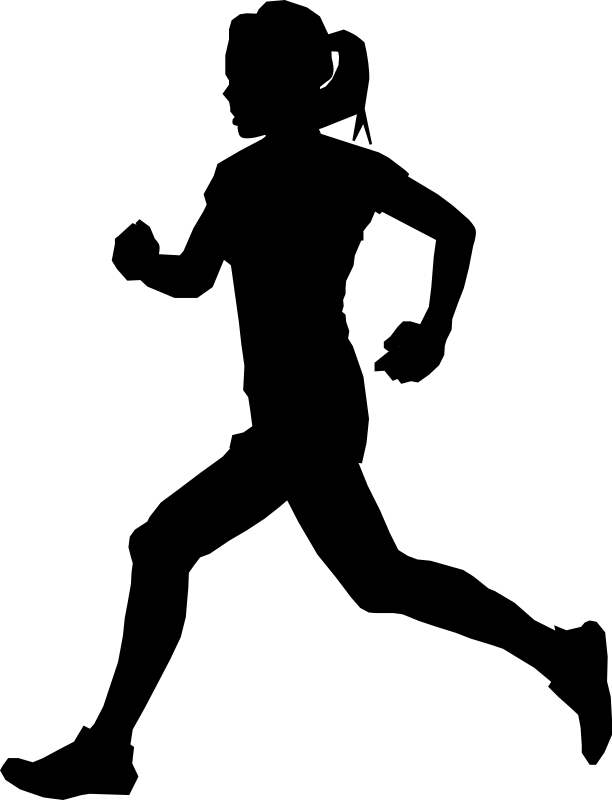
\includegraphics[width=2cm]{pics/runner.png}
    Runners
    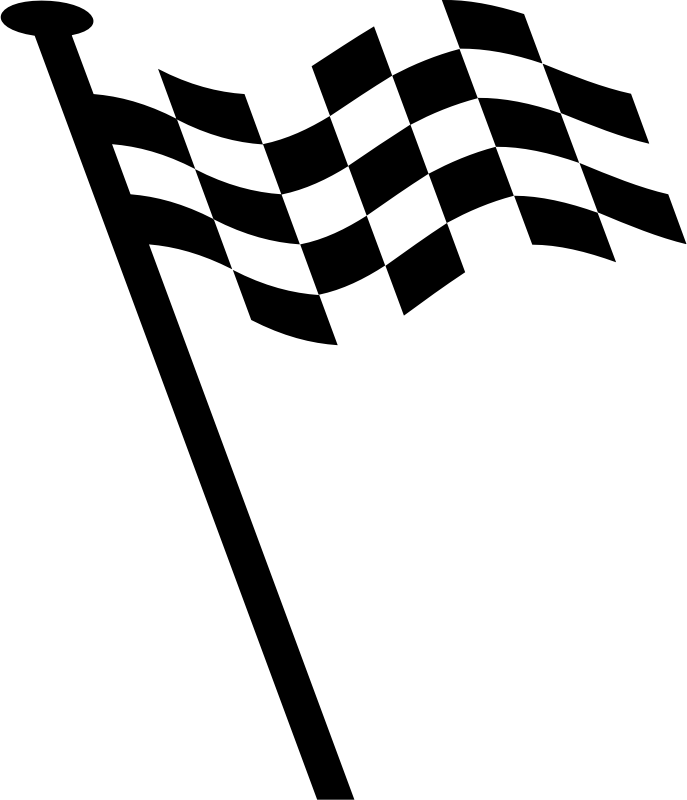
\includegraphics[width=2cm]{pics/race.png}
    Races
    
\includegraphics[width=2cm]{pics/registration.png}
    Registrations
  \end{center}
\end{frame}

\begin{frame}[fragile]
  \frametitle{Typeclasses need laws}
  \begin{itemize}
  \item<1-> typeclasses should \textit{always} come with laws
  \item<1-> what about \texttt{RunnerAlg}?
  \end{itemize}
\begin{minted}{scala}
trait RunnerAlg[F[_]] {
  def saveRunner(runner: Runner): F[Unit]
  def findRunner(id: RunnerId): F[Option[Runner]]
  def listRunner: F[Vector[Runner]]
}
\end{minted}
  \begin{itemize}
  \item<2-> \texttt{saveRunner *> saveRunner}
  \item<2-> \texttt{findRunner *> findRunner}
  \item<2-> \texttt{saveRunner *> findRunner}
  \item<2-> \texttt{saveRunner *> listRunners}
  \end{itemize}
\end{frame}

\begin{frame}[fragile]
  \frametitle{ScalaCheck}
  \begin{itemize}
  \item ScalaCheck is perfect for checking our laws
  \item defined in terms of \texttt{RunnerAlg[F[\_]]}
  \end{itemize}

\begin{minted}{scala}
forAll { (runner: Runner) =>
  run {
    RunnerAlg().saveRunner(runner) *>
      RunnerAlg().findRunner(runner.id)
  }.value should ===(runner)
}
\end{minted}
  \begin{itemize}
  \item instantiate this test for our instances
  \item pure in memory, cassandra, postgres, \dots{}
  \end{itemize}
\end{frame}

\end{document}
